\section{Context Preservation}
\label{sec:eval-context}

The third research question asks how a typographic micro-intervention can change the text while preserving the reader's context.
The eight sessions form a with-and-without comparison: in four of them the context-preserving restore is enabled, and in four it is disabled.
In the enabled condition the restore ran with its highlight cue active, so that condition pairs the positional restore with a brief highlight of the restored sentence (\cref{sec:impl-context}), whereas the disabled condition applies neither; the two are therefore contrasted as a bundle rather than as the restore geometry in isolation, a confound we record in \cref{sec:eval-threats}.
We report two behavioural measures aligned to each intervention, and then the mechanism's own per-intervention record from the four sessions in which it ran.

A regression, a backward saccade against the reading direction, is a standard oculomotor sign of reading disruption \cite{rayner1998eyemovements}.
Because context preservation acts only in the moments after a reflow, we aligned the measures to each intervention rather than averaging over the session: for every applied intervention we measured the reading-resume time, the time to the first forward saccade after it, and the regression rate in the five seconds after it against a matched five-second baseline before it.
The reading-resume time was shorter with preservation than without, with a median of \SI{482}{\milli\second} against \SI{650}{\milli\second} and a mean of \SI{670}{\milli\second} against \SI{923}{\milli\second} (\cref{fig:eval-rrt}).
The regression rate showed the same separation: in the five seconds after an intervention it was 23\% with preservation against 33\% without, having fallen from a 29\% baseline with preservation while staying near its 32\% baseline without (\cref{fig:eval-postreg}).
This pattern held across three-, five-, and ten-second windows, and the resume-time direction held for three of the four participants.
We state the direction of these numbers without drawing an inference from them, as four participants (nineteen interventions with preservation, twenty-six without) do not support one.

\begin{figure}[htbp]
\centering
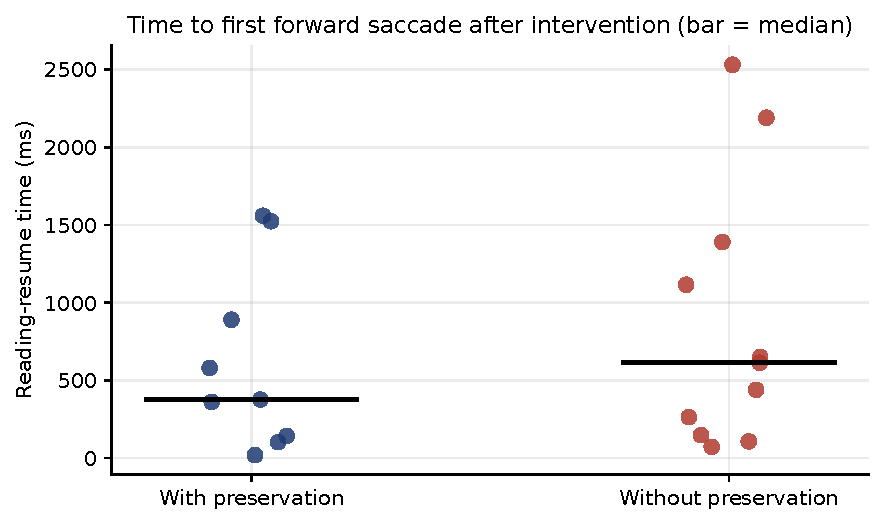
\includegraphics[width=0.7\linewidth]{Chapters/07_Evaluation/eval-rrt.pdf}
\caption[Reading-resume time by condition.]{Reading-resume time, the interval from each intervention to the reader's next forward saccade, under each condition. Each point is one intervention and the horizontal bar marks the median.}
\label{fig:eval-rrt}
\end{figure}

\begin{figure}[htbp]
\centering
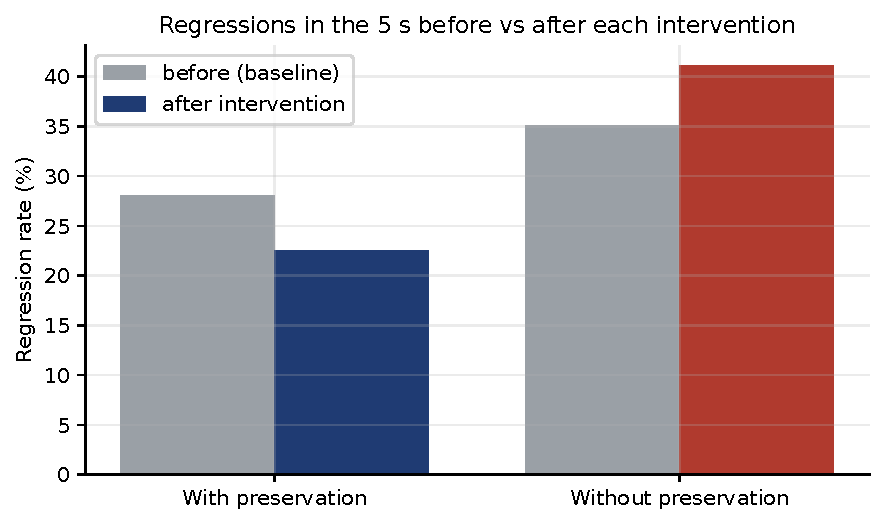
\includegraphics[width=0.7\linewidth]{Chapters/07_Evaluation/eval-post-regression.pdf}
\caption[Regression rate around each intervention.]{Regression rate in the five seconds before and after each intervention, by condition. Without preservation the rate rises after the intervention, whereas with preservation it does not.}
\label{fig:eval-postreg}
\end{figure}

Within the four sessions in which preservation ran, the reader recorded an outcome for each intervention, namely the displacement the reflow induced (the shift of the reader's position before any compensation) and the residual after the restore, together with a graded status.
Most of the nineteen interventions were layout-changing (a font-size, line-width, or line-height change), which trigger the semantic-restart strategy, and one was an appearance-only change.
Three interventions were graded preserved and sixteen degraded.
For the degraded interventions the median residual was 389\,px, while the median induced displacement was only 38\,px.
\Cref{fig:eval-overreposition} plots the residual against the induced displacement for each intervention, and the points lie above the line of equality, that is, the restore moved the reader's position further than the reflow itself had.
This is the measured behaviour of the \emph{original} semantic-restart strategy on small layout reflows; it motivated a revision to the restore that we evaluate with the deterministic sweep below and examine further in \cref{ch:discussion}.
Each outcome, including its graded status, is written into the session record, so the cost of every intervention to the reader's continuity is auditable after the fact.

\begin{figure}[htbp]
\centering
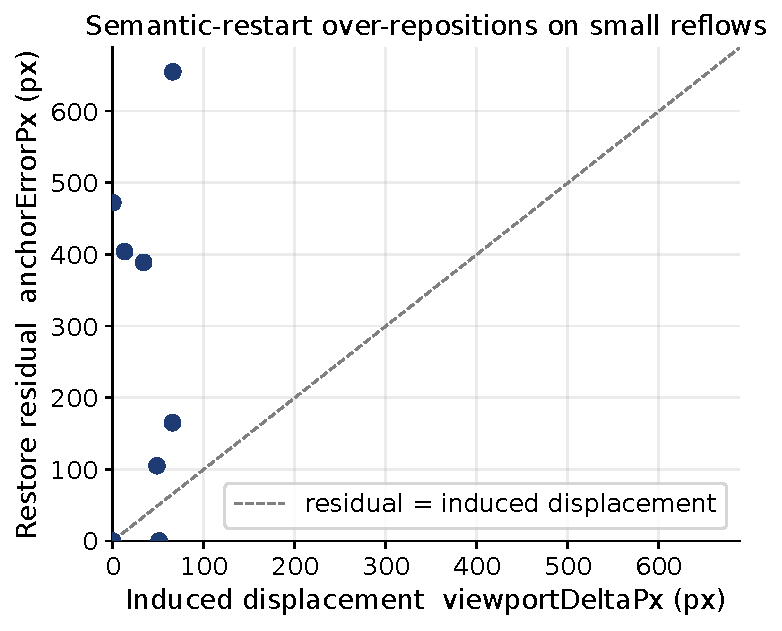
\includegraphics[width=0.68\linewidth]{Chapters/07_Evaluation/eval-restore-overreposition.pdf}
\caption[Restore residual against induced displacement.]{Restore residual against the displacement the reflow induced, with one point per intervention in the four preservation-enabled sessions. Points above the dashed line of equality indicate that the restore repositioned the reader further than the reflow had moved them.}
\label{fig:eval-overreposition}
\end{figure}

The per-intervention record above is observational: each outcome comes from whichever interventions the four participants happened to receive, so it covers neither every intervention type nor a controlled range of magnitudes.
To characterise the displacement a reflow induces independently of which interventions a session happened to apply, we drove the same restore mechanism over a deterministic sweep.
A measurement harness mounts the participant reader (\cref{sec:impl-context}) outside a live session, renders the reading document at the baseline typography, and fires each built-in layout intervention from every page of the paginated document, reading back the values the restore hook emits.
Because the harness exercises the same \idtt{usePreserveReadingContext} path as a live session, the induced displacement and the residual it reports are the mechanism's own rather than a reimplementation, and the harness and its analysis are committed with the source so the figures are reproducible.
The eleven layout interventions crossed with six reading positions yield 66 trials.

\Cref{tab:eval-displacement} reports, for each intervention, the displacement the reflow induced at the reader's position before any compensation, in pixels and in baseline reading lines (one line is \SI{32.4}{px} at the baseline typography).
The median induced displacement was \SI{32.4}{px}, exactly one reading line, and the distribution was strongly intervention-dependent: a six-point font enlargement moved the reading position by a median of 2.73 lines, whereas a line-height increase of 0.3 moved it by 0.08 of a line.
Pooled across interventions the displacement reached \SI{91}{px} at the 95th percentile (about 2.8 lines) and \SI{153}{px} at most (about 4.7 lines).
This central value is of the same order as the \SI{38}{px} median induced displacement measured from the live sessions above, so the controlled sweep and the observational record agree on the scale of the disruption the mechanism must absorb.

Run against the original restore strategy, the sweep reproduces the over-repositioning of \cref{fig:eval-overreposition} under controlled conditions.
The reader's position remained on screen in every trial, but the residual after the restore was a median of \SI{138}{px} and only 16 of the 66 outcomes were graded preserved, the restore having moved the position further than the reflow itself had.
We therefore revised the restore so that a layout reflow returns the reader's captured reading position to the on-screen offset it held before the change, rather than re-establishing the committed segment at the top of the reading area (\cref{sec:impl-context}).
Re-running the identical sweep against the revised strategy, the induced displacement of \cref{tab:eval-displacement} is unchanged (the reflow is the same), but the residual after the restore falls to a median of \SI{31}{px}, one reading line, and 61 of the 66 outcomes are graded preserved.
A direct comparison of the relevant word's final position with preservation off and on confirms the change: with the revised restore the word is moved further than the bare reflow in only 4 of 63 trials, against 46 of 62 before, so preservation now holds the reader's position rather than over-shooting it.
The residual that remains is bounded by the sentence granularity at which the anchor is realigned, and line-width changes, which repaginate the document, lie outside what a within-page restore can compensate; we return to both in \cref{ch:discussion}.

\begin{table}[htbp]
\centering
\small
\caption[Induced displacement per intervention from the deterministic sweep.]{Displacement the reflow induced at the reader's position before any compensation, per intervention, from the 66-trial deterministic sweep. The two pixel columns give the median and 95th percentile of the displacement; the lines column expresses the median in baseline reading lines (one line is \SI{32.4}{px}). The final column counts the trials in which the reader's committed position remained on screen after the restore.}
\label{tab:eval-displacement}
\begin{tabular}{l r r r r r}
\toprule
 & & \multicolumn{2}{c}{\textbf{Displacement (px)}} & \textbf{Median} & \textbf{Position} \\
\cmidrule(lr){3-4}
\textbf{Intervention} & \textbf{n} & \textbf{Median} & \textbf{p95} & \textbf{(lines)} & \textbf{on screen} \\
\midrule
Font size $+2$\,px (18\,$\to$\,20)      & 6 & 13.3 & 49.7  & 0.41 & 6/6 \\
Font size $+6$\,px (18\,$\to$\,24)      & 6 & 88.4 & 145.1 & 2.73 & 6/6 \\
Font size $-2$\,px (18\,$\to$\,16)      & 6 & 79.2 & 81.9  & 2.44 & 6/6 \\
Line height $+0.3$ (1.8\,$\to$\,2.1)    & 6 & 2.7  & 35.3  & 0.08 & 6/6 \\
Line height $-0.3$ (1.8\,$\to$\,1.5)    & 6 & 61.3 & 87.0  & 1.89 & 6/6 \\
Line width $-120$\,px (680\,$\to$\,560) & 6 & 16.2 & 32.4  & 0.50 & 6/6 \\
Line width $+80$\,px (680\,$\to$\,760)  & 6 & 64.8 & 64.8  & 2.00 & 6/6 \\
Letter spacing $+0.06$\,em              & 6 & 32.4 & 32.4  & 1.00 & 6/6 \\
Letter spacing $+0.12$\,em              & 6 & 32.4 & 56.7  & 1.00 & 6/6 \\
Font family $\to$ Inter                 & 6 & 31.4 & 55.7  & 0.97 & 6/6 \\
Font family $\to$ Space Grotesk         & 6 & 32.4 & 56.7  & 1.00 & 6/6 \\
\midrule
\textbf{Overall}                        & 66 & 32.4 & 91.0 & 1.00 & 66/66 \\
\bottomrule
\end{tabular}
\end{table}
